\subsubsection{Documentations and Tutorials}

In this part, we will elaborate on our work in the aspects of documentation and tutorial guidance. 

\begin{enumerate}[(i)]
\item Documentation

First, we mentioned earlier that we collected the requirements table through interviews during sprint1. Here, we classify, merge, and summarize these requirements into a form of documentation. We classify according to the type of requirement, and categorize them into functional requirements and non-functional requirements. We also revise the descriptions and reasons for some requirements to make them more clear and understandable. 

In addition to the requirement documents, we have also organized interface documents. This document was originally used at the coding stage to facilitate members' understanding of the input, output, and functionality of interfaces. However, in the development stage, we made minor adjustments to some of these interfaces (because the design of the interface was not perfect), so we updated the modified interfaces and their functional descriptions into the document. At the same time, we have also compiled our program's structure and logical design into text and graphics, which will be explained in further detail in the solution section.

\item Tutorials

Initially, we added the tutorial as a non-functional requirement in our requirements, as a way to instruct our users on how to use the system more clearly, and outlined it into a document. Therefore, we included it in our sprint3, and if time allowed, we planned to complete this document in the last stage. However, due to time constraints, we could only highlight key widgets on the interface, and use UI elements and other visual components to implicitly instruct users on how to use the system.

\end{enumerate}

\subsubsection{Security Consideration} 

This section mainly discusses the non-functional requirements regarding system security. Since this section is about the protection of software information, it's handled by the two members of the backend team. In this section, we primarily focus on two aspects of security issues, one being the protection of user information within the system, and the other being the resistance to external intrusions. We will briefly introduce our work in these two areas below. A more detailed description on this topic will occur in the section on Security Assessment.

\begin{enumerate}[(i)]
  \item External Invasion

Because our system has a form submission operation, we have implemented a filter check on user input information to prevent external SQL code injections and protect user information. Though our system inherently has the function of detecting SQL code injection, we were considering executing it through calling internal algorithm modules. However, due to time constraints, technical debt was incurred here, and we placed the corresponding detection code in the backend instead of making a better module separation.

  \item Internal Data Management in the System

In terms of user information protection, we executed three main tasks, which included log desensitization detection, password protection, and user information verification. On one hand, we used various methods including hashing, password salting, and digital signatures, to encrypt user information in order to prevent potential attacks such as man-in-the-middle and dictionary attacks, thus enhancing the system's consistency and confidentiality. On the other hand, we carried out desensitization operations on the logs and masked the important information in them to prevent potential internal attacks, fulfilling a non-functional requirement.
\end{enumerate}

\subsubsection{Scalability and Performance} 
Regarding the system's scalability and performance, we mainly consider this issue on the algorithm side. Since our algorithm system is implemented based on an existing open-source system, it lacks code documentation. This leads to inevitable technical debt and refactoring when adding new features due to misunderstandings of the structure. Consequently, the main responsibility for handling this issue falls on the three members of the algorithm group. As for scalability, we mainly consider the following concerns: If a new detection language is added to the system, would the process be complicated? If different detection types are added to the system, will they affect other modules, and will they violate the OCP (Open/Closed Principle)? To address these issues, we have readjusted the underlying structure. At the same time, we resolved the technical debt incurred previously due to the forced addition of java and js modules to ensure the smooth operation of the software.

\subsubsection{Software Structure Optimization}
This part will be explained in greater detail in the solution section, which describes the overall software module structure and operation logic. As shown in Image 1, the original structure was a sequential structure. We made several optimizations to it:
\begin{itemize}
\item Modularization: We divided the original system into multiple sub-modules, making each module's function simpler and serving a specific purpose. For instance, regarding the Rules class, we encapsulated the language, author, and matching rules information within. We can now hide the information originally stored externally and ensure maximum separation between modules, avoiding OCP issues. If we want to add a new language, we only need to add the corresponding language rules data in the relevant rules database. Similarly, if we want to add custom rules, we only need to add a corresponding rules class.
\item Abstract classes (LSP): We abstracted the original phraser class and detection class into a parent class, with dedicated language interpreters and detectors (e.g. java, js, PHP) as their subclasses. They share the same interface, with the only differences being the language type and processed code. This solves the scalability problem, and when we want to add a new detection language, we only need to implement the corresponding language interpreter, detector, and rules, thereby improving system extensibility.
\item Generic middle connection: To reduce the workload of the intermediary connection layer, we minimized the usage of code like \verb|if (code.lang == "java")|. Instead, we looped through the rules array, finding the matched code language rules, and then exporting the corresponding rules. By using a generic method, we reduced the use of conditional statements and made it more convenient to add new rules and detection languages, thereby improving system scalability.
\end{itemize}

\subsubsection{Technical Debt}
Initially, to ensure the smooth operation of the software, we incurred technical debt when adding the Java and Js languages. As shown in Fig.\ref{fig:tdprocess}, we simply placed this part of the code in a branch without integrating it into the original system, Fig.\ref{fig:originprocess}. When there was input, we used an if statement to determine whether it was a Java or Js code file. If so, it was directly input into the corresponding branch. This made the software itself more bloated and complicated. For adding a new language, we would have to add new branches, which worsened software extensibility. Therefore, during this sprint, we inserted these languages as subclasses into the original structure, refactoring the software.

\begin{figure}[h]
  \centering
  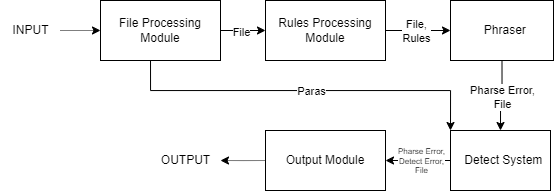
\includegraphics[width=3.3in]{figures/originprocess.png}
  \caption{Origin Process}
  \label{fig:originprocess}
  \end{figure}

  \begin{figure}[h]
    \centering
    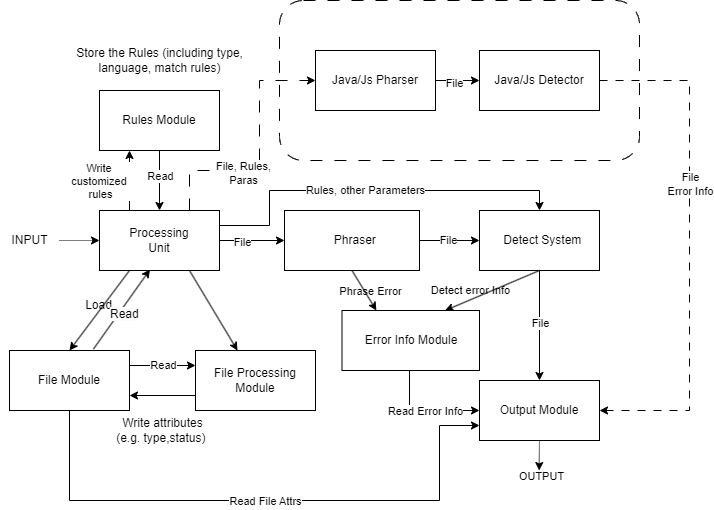
\includegraphics[width=3.3in]{figures/tdprocess.png}
    \caption{TD Process}
    \label{fig:tdprocess}
    \end{figure}

\subsubsection{Testing and Deployment}
In the final part of this sprint, we mainly continue to address the non-functional requirements of the software, such as its maintainability, runtime efficiency, thread-safety, and performance under stress testing.

First, we deployed the software on a server (see the Security Assessment chapter for server configuration details) to facilitate developer access, use, and testing, thus improving system maintainability. We only need to update the code locally and regularly deploy the new program to the server to form new versions, making maintenance work easier for developers. In addition, to assess the efficiency of the detection software, we evaluate whether the system can quickly respond to user needs and provide corresponding code detection from various perspectives, including runtime efficiency, transaction throughput, success rate, and response time. At the same time, we conducted load and stress tests on the system to assess its performance under high-data-volume and multi-threaded testing conditions. Since we had previously focused on unit tests, ensuring the performance of individual modules, we couldn't guarantee that situations such as deadlocks wouldn't occur under multi-threaded conditions or verify the software's efficiency during concurrent situations. Therefore, we verified the software's performance in these aspects through stress and load tests.